\subsection{Pantalla: Iniciar Sesión}
\subsubsection{Objetivo}
	El mapa de navegación se muestra en la Figura~\ref{fig:mapaNavegacionCU0}

   \begin{figure}[hbpt!]
 		\centering
 			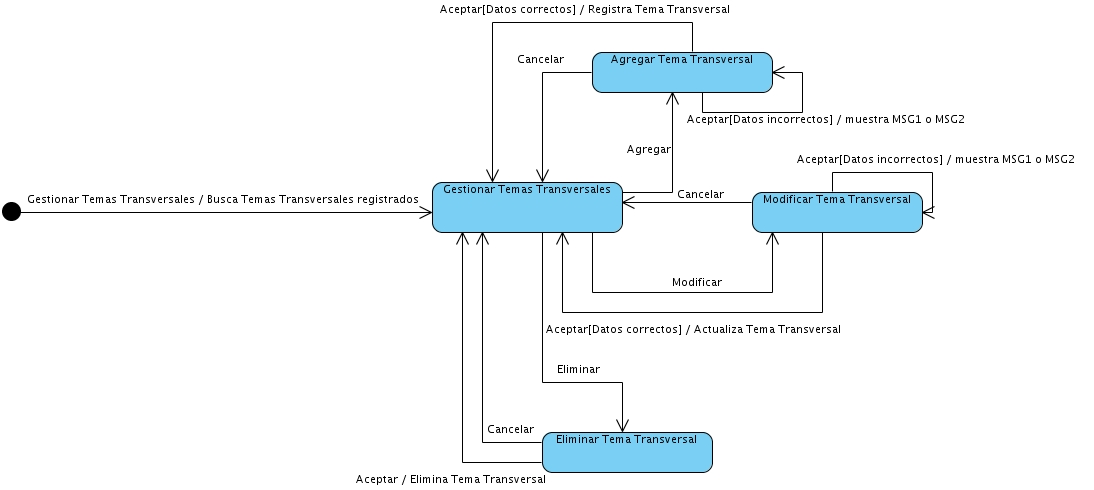
\includegraphics[width=0.8\textwidth]{images/cu0/MapaNavegacion.jpg}
 		\caption{Mapa de navegacion para el CU0 Iniciar Sesión.}
		\label{fig:mapaNavegacionCU0}
 	\end{figure}
\subsubsection{Objetivo}
Iniciar sesión en el sistema.Vease Figura~\ref{IULoggueo}

\IUfig[0.6]{cu0/iniciarsesion.png}{IULoggueo}{Iniciar Sesión.}

\subsubsection{Entradas}
Datos del usuario para iniciar sesión.
\begin{itemize}
\item Login de usuario.(En la pantalla de acceso al sistema el Login de usuario se muestra como ``usuario registrado'', cabe mencionar que hacen referencia a lo mismo).
\item Contraseña de usuario.
\end{itemize}

\subsubsection{Controles}
\begin{itemize}
 \item Se encuentra un \textit{textbox} para ingresar el login del usuario.
 \item Se encuentra un \textit{textbox} para ingresar la contraseña del usuario.
\end{itemize}

\subsubsection{Comandos}
\begin{itemize}
 \item \IUbutton{Aceptar} Inicia la sesión del usuario.

\end{itemize}

\subsubsection{Salidas}
Se muestra el menú de sesión iniciada de acuerdo al perfil del usuario:
\begin{itemize}
 \item Menú para usuarios que cuenten con el perfil de Administrador. Véase Figura~\ref{IUMenuAdministrador}.
	\IUfig[0.3]{cu0/MenuAdministrador.png}{IUMenuAdministrador}{Menú del perfil del Administrador.}

 \item Menú para usuarios que cuenten con el perfil de Gerente. Véase Figura~\ref{IUMenuGerente}.
	\IUfig[0.3]{cu0/MenuGerente.png}{IUMenuGerente}{Menú del perfil de Gerente.}

 \item Menú para usuarios que cuenten con un perfil de Coordinador. Véase Figura~\ref{IUMenuCoordinador}.
	\IUfig[0.3]{cu0/MenuCoordinador.png}{IUMenuCoordinador}{Menú del perfil de Coordinador.}

 \item Menú para usuarios que cuenten con un perfil de Director. Véase Figura~\ref{IUMenuDirector}.
	\IUfig[0.3]{cu0/MenuDirector.png}{IUMenuDirector}{Menú del perfil de Director.}
	
\item Menú para usuarios que cuenten con un perfil de Secretario. Véase Figura~\ref{IUMenuSecretario}.
	\IUfig[0.3]{cu0/MenuSecretaria.png}{IUMenuSecretario}{Menú del perfil de Secretario.}

\end{itemize}

%En la Figura~ \ref{IUMenuDirector} se muestra el menú para el usuario que cuente con un perfil de Gerenter.








%\IUfig[0.8]{cu0/MenuGerente.png}{IUMenuGerente}{Menú para Gerentes.}

% \begin{figure}[hbpt!]
%  		\centering
%  			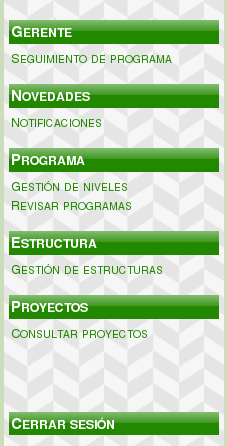
\includegraphics[width=0.8\textwidth]{images/cu0/MenuGerente.png}
%  		\caption{Menú para Gerentes.}
%  		\label{IUMenuGerente}
% \end{figure}






